\section{Structure and Contributions}
\label{sec:introduction-structure}

\subsection{The Implementation Library}
\label{subsec:introduction-structure-library}

\begin{figure}
  \centering
  \definecolor{plantucolor0000}{RGB}{254,254,206}
\definecolor{plantucolor0001}{RGB}{168,0,54}
\definecolor{plantucolor0002}{RGB}{180,167,229}
\definecolor{plantucolor0003}{RGB}{0,0,0}
\definecolor{plantucolor0004}{RGB}{132,190,132}
\definecolor{plantucolor0005}{RGB}{3,128,72}
\definecolor{plantucolor0006}{RGB}{173,209,178}

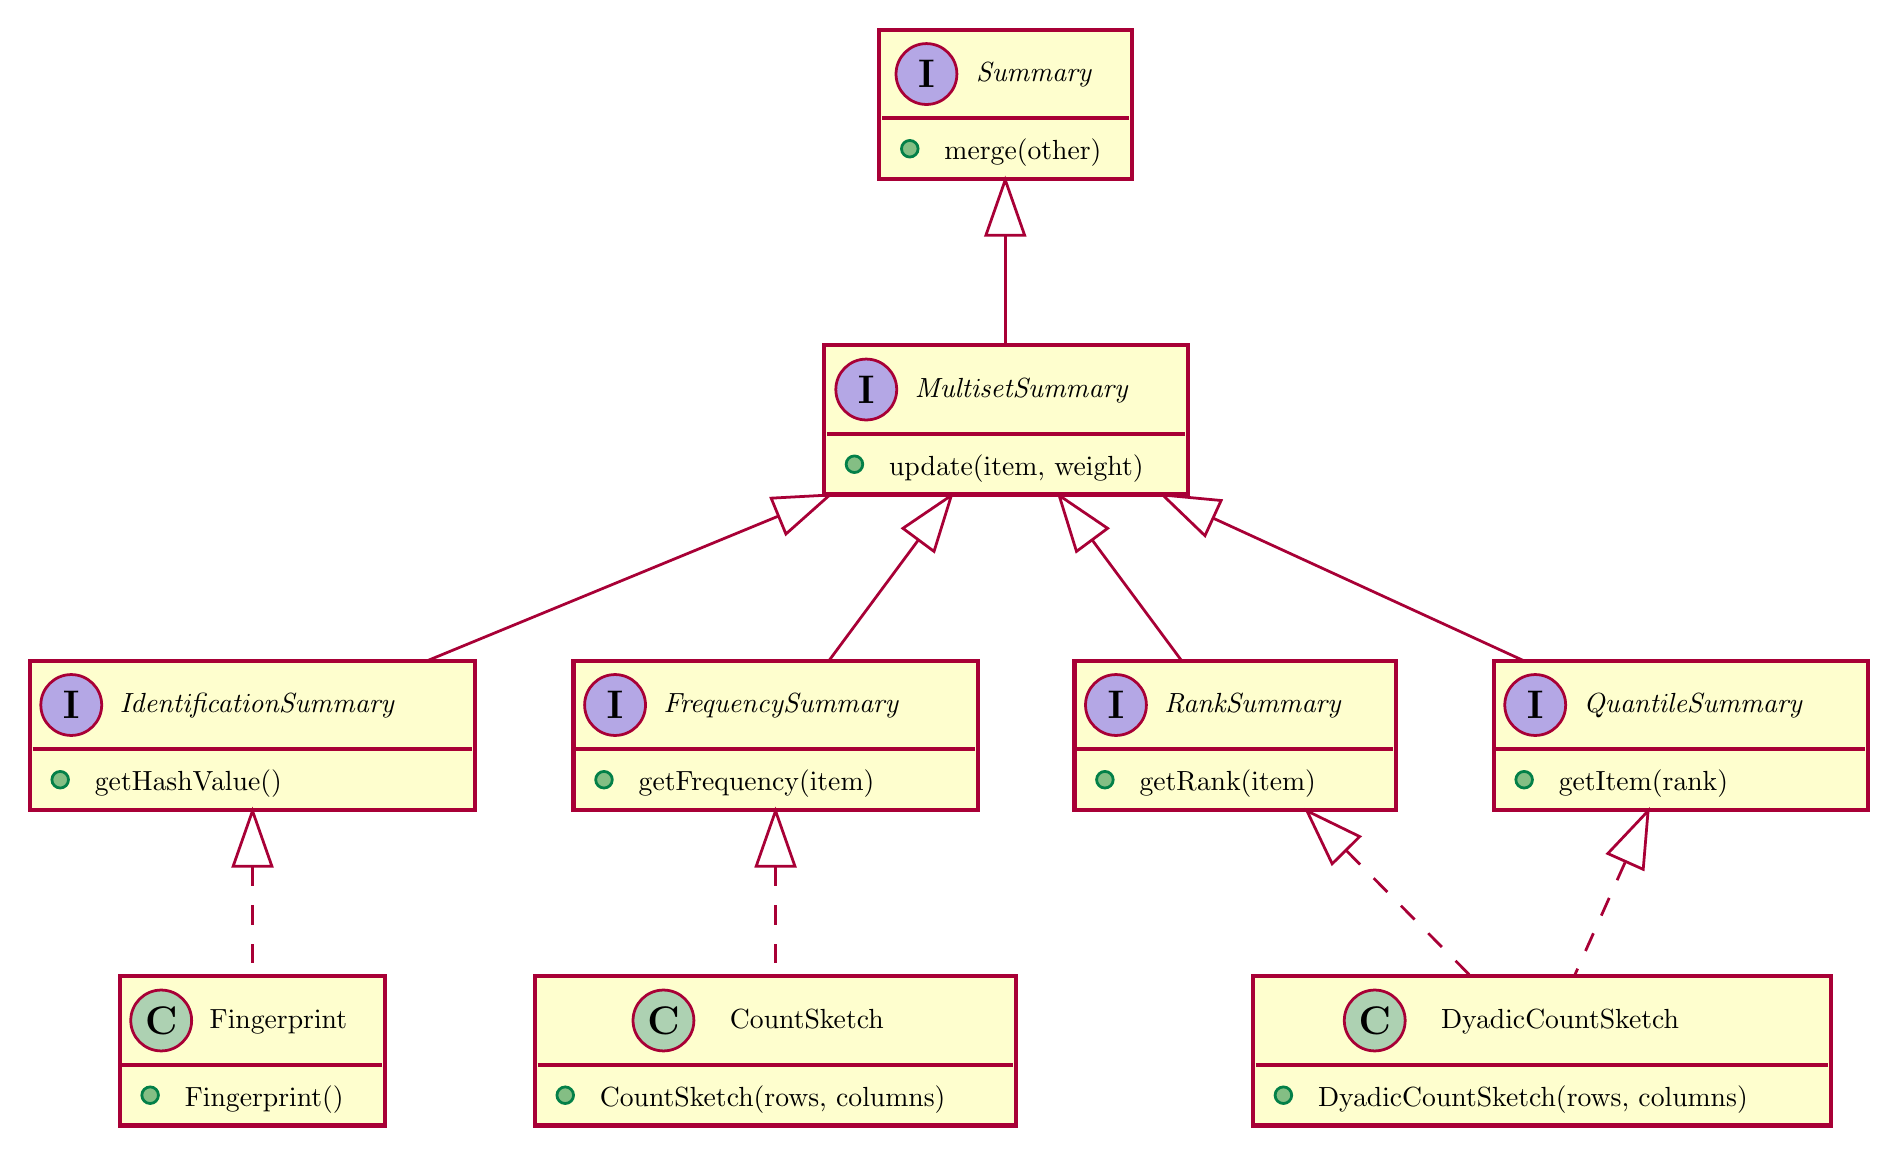
\begin{tikzpicture}[
  yscale=-1,
  pstyle0/.style={color=plantucolor0001,fill=plantucolor0000,line width=1.5pt},
  pstyle1/.style={color=plantucolor0001,fill=plantucolor0002,line width=1.0pt},
  pstyle2/.style={color=plantucolor0001,line width=1.5pt},
  pstyle3/.style={color=plantucolor0005,fill=plantucolor0004,line width=1.0pt},
  pstyle4/.style={color=plantucolor0001,fill=plantucolor0006,line width=1.0pt},
  pstyle5/.style={color=plantucolor0001,line width=1.0pt},
  pstyle6/.style={color=plantucolor0001,line width=1.0pt,dash pattern=on 7.0pt off 7.0pt},
]
  \action<2->{
    \draw[pstyle0] (314pt,7pt) rectangle (405.2656pt,60.9434pt);
    \draw[pstyle1] (331.0252pt,23pt) ellipse (11pt and 11pt);
    \node at (331.0252pt,23pt)[]{\textbf{\Large I}};
    \node at (345.4752pt,15.3945pt)[below right,color=black]{\textit{Summary}};
    \draw[pstyle2] (315pt,39pt) -- (404.2656pt,39pt);
    \draw[pstyle3] (325pt,50pt) ellipse (3pt and 3pt);
    \node at (334pt,43pt)[below right,color=black]{merge(other)};
  }
  \action<3->{
    \draw[pstyle0] (294pt,121pt) rectangle (425.4105pt,174.9434pt);
    \draw[pstyle1] (309.2747pt,137pt) ellipse (11pt and 11pt);
    \node at (309.2747pt,137pt)[]{\textbf{\Large I}};
    \node at (323.3358pt,129.3945pt)[below right,color=black]{\textit{MultisetSummary}};
    \draw[pstyle2] (295pt,153pt) -- (424.4105pt,153pt);
    \draw[pstyle3] (305pt,164pt) ellipse (3pt and 3pt);
    \node at (314pt,157pt)[below right,color=black]{update(item, weight)};
  }
  \action<4->{
    \draw[pstyle0] (7pt,235pt) rectangle (167.9704pt,288.9434pt);
    \draw[pstyle1] (22pt,251pt) ellipse (11pt and 11pt);
    \node at (22pt,251pt)[]{\textbf{\Large I}};
    \node at (36pt,243.3945pt)[below right,color=black]{\textit{IdentificationSummary}};
    \draw[pstyle2] (8pt,267pt) -- (166.9704pt,267pt);
    \draw[pstyle3] (18pt,278pt) ellipse (3pt and 3pt);
    \node at (27pt,271pt)[below right,color=black]{getHashValue()};
    \draw[pstyle0] (203.5pt,235pt) rectangle (349.5333pt,288.9434pt);
    \draw[pstyle1] (218.5pt,251pt) ellipse (11pt and 11pt);
    \node at (218.5pt,251pt)[]{\textbf{\Large I}};
    \node at (232.5pt,243.3945pt)[below right,color=black]{\textit{FrequencySummary}};
    \draw[pstyle2] (204.5pt,267pt) -- (348.5333pt,267pt);
    \draw[pstyle3] (214.5pt,278pt) ellipse (3pt and 3pt);
    \node at (223.5pt,271pt)[below right,color=black]{getFrequency(item)};
    \draw[pstyle0] (384.5pt,235pt) rectangle (500.5732pt,288.9434pt);
    \draw[pstyle1] (399.5pt,251pt) ellipse (11pt and 11pt);
    \node at (399.5pt,251pt)[]{\textbf{\Large I}};
    \node at (413.5pt,243.3945pt)[below right,color=black]{\textit{RankSummary}};
    \draw[pstyle2] (385.5pt,267pt) -- (499.5732pt,267pt);
    \draw[pstyle3] (395.5pt,278pt) ellipse (3pt and 3pt);
    \node at (404.5pt,271pt)[below right,color=black]{getRank(item)};
    \draw[pstyle0] (536pt,235pt) rectangle (671.2046pt,288.9434pt);
    \draw[pstyle1] (551pt,251pt) ellipse (11pt and 11pt);
    \node at (551pt,251pt)[]{\textbf{\Large I}};
    \node at (565pt,243.3945pt)[below right,color=black]{\textit{QuantileSummary}};
    \draw[pstyle2] (537pt,267pt) -- (670.2046pt,267pt);
    \draw[pstyle3] (547pt,278pt) ellipse (3pt and 3pt);
    \node at (556pt,271pt)[below right,color=black]{getItem(rank)};
  }
  \action<5->{
    \draw[pstyle0] (39.5pt,349pt) rectangle (135.263pt,402.9434pt);
    \draw[pstyle4] (54.5pt,365pt) ellipse (11pt and 11pt);
    \node at (54.5pt,365pt)[]{\textbf{\Large C}};
    \node at (68.5pt,357.3945pt)[below right,color=black]{Fingerprint};
    \draw[pstyle2] (40.5pt,381pt) -- (134.263pt,381pt);
    \draw[pstyle3] (50.5pt,392pt) ellipse (3pt and 3pt);
    \node at (59.5pt,385pt)[below right,color=black]{Fingerprint()};
    \draw[pstyle0] (189.5pt,349pt) rectangle (363.4455pt,402.9434pt);
    \draw[pstyle4] (235.9905pt,365pt) ellipse (11pt and 11pt);
    \node at (235.9905pt,365pt)[]{\textbf{\Large C}};
    \node at (256.4905pt,357.3945pt)[below right,color=black]{CountSketch};
    \draw[pstyle2] (190.5pt,381pt) -- (362.4455pt,381pt);
    \draw[pstyle3] (200.5pt,392pt) ellipse (3pt and 3pt);
    \node at (209.5pt,385pt)[below right,color=black]{CountSketch(rows, columns)};
    \draw[pstyle0] (449pt,349pt) rectangle (657.8976pt,402.9434pt);
    \draw[pstyle4] (493.0053pt,365pt) ellipse (11pt and 11pt);
    \node at (493.0053pt,365pt)[]{\textbf{\Large C}};
    \node at (513.451pt,357.3945pt)[below right,color=black]{DyadicCountSketch};
    \draw[pstyle2] (450pt,381pt) -- (656.8976pt,381pt);
    \draw[pstyle3] (460pt,392pt) ellipse (3pt and 3pt);
    \node at (469pt,385pt)[below right,color=black]{DyadicCountSketch(rows, columns)};
  }
  \action<3->{
    \draw[pstyle5] (359.5pt,81.37pt) ..controls (359.5pt,94.87pt) and (359.5pt,109.13pt) .. (359.5pt,120.91pt);
    \draw[pstyle5] (352.5pt,81.26pt) -- (359.5pt,61.26pt) -- (366.5pt,81.26pt) -- (352.5pt,81.26pt) -- cycle;
  }
  \action<4->{
    \draw[pstyle5] (277.45pt,182.78pt) ..controls (236.91pt,199.48pt) and (188.72pt,219.32pt) .. (151.03pt,234.84pt);
    \draw[pstyle5] (274.91pt,176.26pt) -- (296.07pt,175.12pt) -- (280.24pt,189.21pt) -- (274.91pt,176.26pt) -- cycle;
    \draw[pstyle5] (327.98pt,191.53pt) ..controls (317.17pt,206.12pt) and (305.39pt,222.01pt) .. (295.84pt,234.91pt);
    \draw[pstyle5] (322.51pt,187.16pt) -- (340.04pt,175.26pt) -- (333.76pt,195.5pt) -- (322.51pt,187.16pt) -- cycle;
    \draw[pstyle5] (391.02pt,191.53pt) ..controls (401.83pt,206.12pt) and (413.61pt,222.01pt) .. (423.16pt,234.91pt);
    \draw[pstyle5] (385.24pt,195.5pt) -- (378.96pt,175.26pt) -- (396.49pt,187.16pt) -- (385.24pt,195.5pt) -- cycle;
    \draw[pstyle5] (434.59pt,183.47pt) ..controls (470.65pt,200.02pt) and (513.16pt,219.53pt) .. (546.51pt,234.84pt);
    \draw[pstyle5] (431.66pt,189.82pt) -- (416.4pt,175.12pt) -- (437.5pt,177.1pt) -- (431.66pt,189.82pt) -- cycle;
  }
  \action<5->{
    \draw[pstyle6] (87.5pt,309.37pt) ..controls (87.5pt,322.87pt) and (87.5pt,337.13pt) .. (87.5pt,348.91pt);
    \draw[pstyle5] (80.5pt,309.26pt) -- (87.5pt,289.26pt) -- (94.5pt,309.26pt) -- (80.5pt,309.26pt) -- cycle;
    \draw[pstyle6] (276.5pt,309.37pt) ..controls (276.5pt,322.87pt) and (276.5pt,337.13pt) .. (276.5pt,348.91pt);
    \draw[pstyle5] (269.5pt,309.26pt) -- (276.5pt,289.26pt) -- (283.5pt,309.26pt) -- (269.5pt,309.26pt) -- cycle;
    \draw[pstyle6] (482.78pt,303.64pt) ..controls (497.74pt,318.74pt) and (514.3pt,335.45pt) .. (527.64pt,348.91pt);
    \draw[pstyle5] (477.63pt,308.39pt) -- (468.52pt,289.26pt) -- (487.58pt,298.54pt) -- (477.63pt,308.39pt) -- cycle;
    \draw[pstyle6] (583.44pt,307.92pt) ..controls (577.23pt,321.84pt) and (570.59pt,336.71pt) .. (565.15pt,348.91pt);
    \draw[pstyle5] (577.23pt,304.67pt) -- (591.78pt,289.26pt) -- (590.02pt,310.38pt) -- (577.23pt,304.67pt) -- cycle;
  }
\end{tikzpicture}
%
  \caption{Abridged class diagram of the \lstinline{summaries} package}
  \label{fig:introduction-structure-library-summaries}
\end{figure}

The structure of the main \lstinline{summaries} package is shown in \cref{fig:introduction-structure-library-summaries}.
This abridged class diagram omits the helper methods and utility classes that are described in the implementation sections of each summary chapter.
The four operations common to all of the summaries studied in this project are
\begin{enumerate*}
  \item initialization, which sets the summary to its initial state;
  \item update, which accepts a new datum from the stream and updates its summary of the data accordingly;
  \item merge, which allows two summaries computed over distinct portions of the data to be combined; and
  \item query, which returns the property of the data maintained by a particular summary.
\end{enumerate*}
The \lstinline{Summary} interface declares three abstract methods that are common to all implemented summaries.
The \lstinline{merge} method corresponds to the merge operation of the summary, whereas the \lstinline{copy} and \lstinline{reset} methods do not correspond to operations described in literature, but exist instead to aid the development of wrapper classes such as implementations of Apache~Spark's \lstinline{AccumulatorV2}, which expects this functionality to be available~\citep{tasf14}.
The \lstinline{MultisetSummary} interface extends \lstinline{Summary} and declares an abstract \lstinline{update} method that corresponds to the update operation of the summary.
This method accepts an integer item and an integer weight.
Thus, it is specific to summaries of integer multiset data.
Placing this method in a separate interface allows for summaries of other types of data to extend the \lstinline{Summary} interface.
For example, a summary of standard set data would not require a weight parameter in its update method, and counters such as the Morris counter do not require any update parameters at all~\citep{cormode20,morris78}.
The \lstinline{IdentificationSummary}, \lstinline{FrequencySummary}, \lstinline{RankSummary} and \lstinline{QuantileSummary} interfaces extend \lstinline{MultisetSummary} to provide query methods for their corresponding classes of summary (see \cref{sec:introduction-aims}).
This is necessary because different summaries require different parameters for queries and return different values.
For example, the query method of an \lstinline{IdentificationSummary} simply returns a hash value of type \lstinline{long}, whereas that of a \lstinline{FrequencySummary} returns the approximate frequency of type \lstinline{int} of an item also of type \lstinline{int} given as an argument.
By giving the query methods different names, summaries may inherit multiple query methods, as is the case for the \lstinline{DyadicCountSketch} class.
The initialization operations are implemented by the constructors of the concrete \lstinline{Fingerprint}, \lstinline{CountSketch} and \lstinline{DyadicCountSketch} classes.

For each summary class, a corresponding wrapper class has been developed to adapt the summary for use in the Apache~Spark stream processing framework as an implementation of \lstinline{AccumulatorV2}, which can be used as a shared variable in a parallel operation on a distributed dataset~\citep{tasf14}.
This allows the performance and accuracy tests to be performed using the existing functionality of Apache~Spark.

\subsection{The Written Work}
\label{subsec:introduction-structure-work}

The structure of the remainder of this text closely reflects the process followed during the project.
It is recommended, therefore, to read each chapter and section in the order presented.
\Cref{ch:fingerprint,ch:count-sketch,ch:dyadic-count-sketch} cover the fingerprint summary, count sketch and dyadic count sketch, respectively.
Each of these chapters is split into the following sections:
\begin{enumerate*}
  \item overview, in which background information and an introductory description of the summary are provided;
  \item theory, in which the operations of the summary are explained and formalized using pseudocode algorithms;
  \item analysis, in which the accuracy, complexity and utility of the summary are discussed; and
  \item implementation and evaluation, in which the Java implementation of the summary and its technicalities are discussed, and the methodology, results and analyses of the tests performed on the implementation are presented.
\end{enumerate*}

For the fingerprint summary and count sketch, the analyses include informal proof sketches of accuracy guarantees that are derived from those found in existing literature.
Although these do not provide any new conclusions, they explicitly state much of the required knowledge that is assumed in the literature, and are presented in a manner more suitable as introductory material for those unfamiliar with probability theory and the analysis of streaming algorithms---of whom the author is one.
For the dyadic count sketch, the proof sketch of the accuracy guarantee is omitted in favour of an original discussion on how the summary can be adapted to summarize extended multisets of both positive and negative integers.
No such discussion was found elsewhere during the literature review.

A discussion of the project itself is presented in \cref{ch:discussion}.
This includes the reasoning behind some of the more interesting decisions made throughout the project, as well as its limitations, and recommendations towards how it could be extended or improved.
For information regarding how to access and make use of the accompanying project repository, see \cref{app:repository}.
The notation used throughout this text is described in \cref{app:notation}.
